% Copyright (C) 2002-2006  Alexei Gilchrist and Paul Cochrane
% 
% This program is free software; you can redistribute it and/or
% modify it under the terms of the GNU General Public License
% as published by the Free Software Foundation; either version 2
% of the License, or (at your option) any later version.
%
% This program is distributed in the hope that it will be useful,
% but WITHOUT ANY WARRANTY; without even the implied warranty of
% MERCHANTABILITY or FITNESS FOR A PARTICULAR PURPOSE.  See the
% GNU General Public License for more details.
%
% You should have received a copy of the GNU General Public License
% along with this program; if not, write to the Free Software
% Foundation, Inc., 59 Temple Place - Suite 330, Boston, MA  02111-1307, USA.

% $Id: pyscriptOptics.tex,v 1.7 2006/06/06 11:33:11 paultcochrane Exp $

\chapter{PyScript Optics Object Package}

This package is a library of functions and objects for use in constructing
optical circuits such as those used in interferometers and optical setups
useful in scientific applications.

\section{Examples}

\subsection{Michelson-Morely Interferometer}

This example shows how to construct one of the simplest interferometers with
\pyscript.  A laser is incident onto a 50:50 beam splitter, the light beam
then being split equally into the two ``arms'' of the interferometer.  At
the end of each arm is a mirror which reflects the light directly back to
the beam splitter which recombines the light, and the output of the
interferometer is measured at the detector (below the beam splitter in the
diagram).  As the length of one of the arms changes the voltage measured at
the detector will vary sinusoidally.  In this example we are using the
\obj{Laser}, \obj{Mirror}, \obj{BSBox} and \obj{Detector} objects of the
\lib{optics} library.

\begin{python}
# Michelson-Morely interferometer

# import the pyscript objects
from pyscript import *
# import the optics library
from pyscript.lib.optics import *

# set up some handy defaults
defaults.units=UNITS['cm']

# initialise a laser beam
beam = Group()

# the laser
laser = Laser(c=P(0,0))

# the beam splitter
bs = BSBox(height=0.7)
bs.w = laser.e + P(1,0)
beam.append(Path(laser.e, bs.w))

# the "north" mirror
mirror_n = Mirror(angle=90)
mirror_n.s = bs.n + P(0,3)
beam.append(Path(bs.n, mirror_n.s))

# the "east" mirror
mirror_e = Mirror()
mirror_e.w = bs.e + P(3,0)
beam.append(Path(bs.e, mirror_e.w))

# the detector
det = Detector(angle=90)
det.n = bs.s + P(0,-1)
beam.append(Path(bs.s, det.n))

# make the beam red
beam.apply(fg=Color("red"))

# collect all the objects together
fig = Group(
        laser,
        bs,
        mirror_n, mirror_e,
        det,
        beam,
        )

# render the figure
render(fig,
        file="michelson-morely.eps")
\end{python}

\begin{figure}[ht]
\centerline{\includegraphics[width=\figwidth]{optics/michelson-morely}}
\caption{Michelson-Morely interferometer}
\label{fig:michelson-morely}
\end{figure}

\subsection{Mach-Zehnder Interferometer}

Another commonly used interferometer is the Mach-Zehnder interferometer.  In
this design there are two beam splitters.  The light is split on the first
beam splitter, and travels down each arm of the interferometer to two
mirrors which recombine the light on the second beam splitter, the output
being detected by two detectors at the two output ports of the second beam
splitter.  This interferometer is commonly used for explaining such concepts
as Quantum Non-Demolition experiments, and other ``quantum weirdness''
associated with light.

\begin{python}
# Mach-Zehnder interferometer

# import the pyscript objects
from pyscript import *
# import the optics library
from pyscript.lib.optics import *

# set up some handy defaults
defaults.units=UNITS['cm']

# initialise a laser beam
beam = Group()

# the laser
laser = Laser(c=P(0,0))

# the "west" beam splitter
bs_w = BSBox(height=0.7)
bs_w.w = laser.e + P(1,0)
beam.append(Path(laser.e, bs_w.w))

# the "north" mirror
mirror_n = Mirror(angle=45)
mirror_n.s = bs_w.n + P(0,3)
beam.append(Path(bs_w.n, mirror_n.c))

# the "east" mirror
mirror_e = Mirror(angle=45)
mirror_e.w = bs_w.e + P(3,0)
beam.append(Path(bs_w.e, mirror_e.c))

# the "east" beam splitter
bs_e = BSBox(height=0.7)
bs_e.c = P(mirror_e.c.x, mirror_n.c.y)
beam.append(Path(mirror_e.c, bs_e.s))
beam.append(Path(mirror_n.c, bs_e.w))

# the "north" detector
det_n = Detector(angle=-90)
det_n.s = bs_e.n + P(0,1)
beam.append(Path(bs_e.n, det_n.s))

# the "east" detector
det_e = Detector()
det_e.w = bs_e.e + P(1,0)
beam.append(Path(bs_e.e, det_e.w))

# set the colour of the beam
beam.apply(fg=Color("red"))

# collect all the objects together
fig = Group(
        laser,
        bs_w,
        mirror_n, mirror_e,
        bs_e,
        det_n, det_e,
        beam,
        )

# render the figure
render(fig,
        file="mach-zehnder.eps")
\end{python}

\begin{figure}[ht]
\centerline{\includegraphics[width=\figwidth]{optics/mach-zehnder}}
\caption{Mach-Zehnder interferometer}
\label{fig:mach-zehnder}
\end{figure}

\subsection{Sagnac Interferometer}

The Sagnac interferometer is another of the major interferometer
configurations.  The light is split on the beam splitter and procedes around
the interferometer in opposite directions then being recombined on the same
beam splitter and the output interference is read at the output port (where
the detector is in the diagram  This interferometer can be used in optical
gyroscopes because a rotation in the plane of the interferometer can be
measured since the light traveling in one direction travels a different
distance to the light traveling in the other direction, hence giving a path
difference and interference fringes.  An interesting point about the script
below is that the ``north-east'' mirror has its location set by the y
position of the centre of the ``north'' mirror and its x position set by the
centre of the ``east'' mirror.  This means that if one changes the location
of either of these two mirrors then the position of the ``north-east''
mirror changes appropriately.

\begin{python}
# Sagnac interferometer

# import the pyscript objects
from pyscript import *
# import the optics library
from pyscript.lib.optics import *

# set up some handy defaults
defaults.units=UNITS['cm']

# initialise a laser beam
beam = Group()

# the laser
laser = Laser(c=P(0,0))

# the beam splitter
bs = BSBox(height=0.7)
bs.w = laser.e + P(1,0)
beam.append(Path(laser.e, bs.w))

# the "north" mirror
mirror_n = Mirror(angle=45)
mirror_n.s = bs.n + P(0,2)
beam.append(Path(bs.n, mirror_n.c))

# the "east" mirror
mirror_e = Mirror(angle=45)
mirror_e.w = bs.e + P(3,0)
beam.append(Path(bs.e, mirror_e.c))

# the "north-east" mirror
mirror_ne = Mirror(angle=135)
mirror_ne.c = P(mirror_e.c.x, mirror_n.c.y)
beam.append(Path(mirror_n.c, mirror_ne.c))
beam.append(Path(mirror_e.c, mirror_ne.c))

# the detector
det = Detector(angle=90)
det.n = bs.s + P(0,-1)
beam.append(Path(bs.s, det.n))

# set the colour of the beam
beam.apply(fg=Color("red"))

# collect all the objects together
fig = Group(
        beam,
        laser,
        bs,
        mirror_n, mirror_e, mirror_ne,
        det,
        )

# render the figure
render(fig, 
        file="sagnac.eps")
\end{python}

\begin{figure}[ht]
\centerline{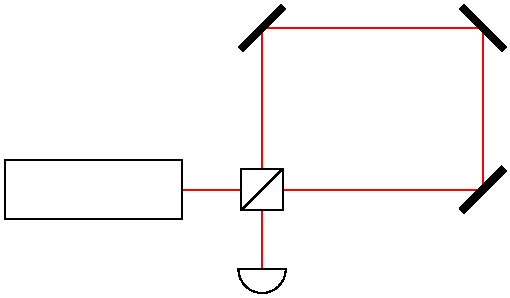
\includegraphics[width=\figwidth]{optics/sagnac}}
\caption{Sagnac interferometer}
\label{fig:sagnac}
\end{figure}

\subsection{A Fabry-Perot Cavity}

A Fabry-Perot cavity is basically just two parallel mirrors facing one
another and a laser field injected into the cavity via one of the mirrors
(which might be 95\% reflective, say).  In the setup shown here we have a
Pound-Drever-Hall setup which can allow for stabilisation of the cavity via
the electro-optical modulator (EOM).  The diagram in
\fig{fig:fabry-perot-pdh} shows such a cavity with a \obj{FreeSpace()}
object used as well.  This is something important for gravitational wave
detectors as they have a lot of free space in the arms of the
interferometers!  Also introduced in this example is the \obj{Modulator()}
object.

\begin{python}
# a Fabry-Perot cavity in a Pound-Drever-Hall setup

# import the pyscript objects
from pyscript import *
# import the optics library
from pyscript.lib.optics import *

# set up some handy defaults
defaults.units=UNITS['cm']

# initialise a laser beam
beam = Group()

# the laser
laser = Laser(c=P(0,0))

# the EOM
eom = Modulator()
eom.w = laser.e + P(1,0)
beam.append(Path(laser.e, eom.w))

# the "west" mirror
mirror_w = Mirror()
mirror_w.w = eom.e + P(1,0)
beam.append(Path(eom.e, mirror_w.w))

# some free space
fs = FreeSpace()
fs.w = mirror_w.e + P(1,0)
beam.append(Path(mirror_w.e, fs.w))

# the "east" mirror
mirror_e = Mirror()
mirror_e.w = fs.e + P(1,0)
beam.append(Path(fs.e, mirror_e.w))

# set the colour of the beam
beam.apply(fg=Color("red"))

# collect all the objects together
fig = Group(
        beam,
        laser,
        eom,
        mirror_e, mirror_w,
        fs,
        )

# render the figure
render(fig,
        file="fabry-perot_pdh.eps")
\end{python}

\begin{figure}[ht]
\centerline{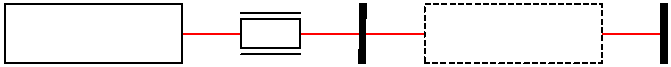
\includegraphics[width=\figwidth]{optics/fabry-perot_pdh}}
\caption{Fabry-Perot cavity in Pound-Drever-Hall setup.}
\label{fig:fabry-perot-pdh}
\end{figure}

\section{Objects}

\subsection{BSBox}

A beam splitter shown as a box.  Some beam splitters are two prisms of glass
bonded together and look like a box with a line along the diagonal
when viewed from above, hence the look of this object.

Object options:
\begin{description}
\item[height:] The height of the beam splitter, its width is equal to its
height.
\item[angle:] Rotation angle.  The beam splitter can be returned already
turned to the desired angle (in degrees).
\item[fg:] The foreground colour.  Use the \obj{Color} object to set this
option.
\item[bg:] The background colour.  Use the \obj{Color} object to set this
option.
\end{description}

\begin{figure}[!ht]
\centerline{\includegraphics[height=1cm]{optics/BSBox}}
\caption{BSBox object}
\label{fig:bsbox}
\end{figure}

\subsection{BSLine}

A beam splitter shown as a thin box at a default angle of 45 degrees.  Some
beam splitters are partially silvered mirrors, hence the look of this
object.

Object options:
\begin{description}
\item[height:] The height of the beam splitter.
\item[thickness:] The thickness of the beam splitter.
\item[angle:] Rotation angle.  The beam splitter can be returned already
turned to the desired angle (in degrees).  The default angle is 45 degrees.
\item[fg:] The foreground colour.  Use the \obj{Color} object to set this
option.
\item[bg:] The background colour.  Use the \obj{Color} object to set this
option.
\end{description}

\begin{figure}[!ht]
\centerline{
\includegraphics[height=1cm]{optics/BSLine}}
\caption{BSLine object}
\label{fig:bsline}
\end{figure}

\subsection{Detector}

A simple D-shaped detector symbol.

Object options:
\begin{description}
\item[height:] The height of the detector
\item[width:] The width of the detector.
\item[angle:] Rotation angle.  The detector can be returned already
turned to the desired angle (in degrees).
\item[pad:] Space padding around the object.
\item[fg:] The foreground colour.  Use the \obj{Color} object to set this
option.
\item[bg:] The background colour.  Use the \obj{Color} object to set this
option.
\end{description}

\begin{figure}[!ht]
\centerline{\includegraphics[height=1cm]{optics/Detector}}
\caption{Detector object}
\label{fig:detector}
\end{figure}

\subsection{Free Space}

This object generates a dashed box where the free space is.  This can be
useful if one wants to highlight that the free space in one arm of an
interferometer has a particular refractive index, or some other property.

Object options:
\begin{description}
\item[height:] The height of the free space region.
\item[width:] The width of the free space region.
\item[angle:] Rotation angle.  
\item[fg:] The foreground colour.  Use the \obj{Color} object to set this
option.
\item[bg:] The background colour.  Use the \obj{Color} object to set this
option.
\end{description}

\begin{figure}[!ht]
\centerline{\includegraphics[height=1cm]{optics/FreeSpace}}
\caption{Free Space object}
\label{fig:free_space}
\end{figure}

\subsection{Lambda Plate}

This object is used to describe changes in an optical beam of, for example,
a half or a quarter of a wavelength.

Object options:
\begin{description}
\item[height:] The height of the lambda plate.
\item[width:] The width of the lambda plate.
\item[angle:] Rotation angle.
\item[fg:] The foreground colour.  Use the \obj{Color} object to set this
option.
\item[bg:] The background colour.  Use the \obj{Color} object to set this
option.
\end{description}

\begin{figure}[!ht]
\centerline{\includegraphics[height=1cm]{optics/LambdaPlate}}
\caption{Lambda Plate object}
\label{fig:lambda_plate}
\end{figure}

\subsection{Laser}

At present all this object does is generate a simple box.  However, in the
future we hope to make this somewhat better looking.

\begin{figure}[!ht]
\centerline{\includegraphics[height=1cm]{optics/Laser}}
\caption{Laser object}
\label{fig:laser}
\end{figure}

\subsection{Lens}

Generate a convex or concave lens.

Object options:
\begin{description}
\item[height:] The height of the lens.
\item[thickness:] The thickness of the lens.
\item[angle:] Rotation angle.
\item[type:] A string specifying if the lens is convex or concave.  Default
is \ttt{concave}.
\item[fg:] The foreground colour.  Use the \obj{Color} object to set this
option.
\item[bg:] The background colour.  Use the \obj{Color} object to set this
option.
\end{description}

\begin{figure}[!ht]
\centerline{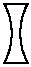
\includegraphics[height=1cm]{optics/Lens}}
\caption{Lens object}
\label{fig:lens}
\end{figure}

\subsection{Mirror}

A very simple mirror symbol.  At present doesn't handle concave/convex
mirrors, but will do hopefully in the future.

Object options:
\begin{description}
\item[length:] The length of the mirror.
\item[thickness:] The thickness of the mirror.
\item[angle:] Rotation angle.
\item[flicks:] Should ``flicks'' indicating the back of the mirror be put
on?  This is a boolean value, and by default this is \ttt{False}.
\item[fg:] The foreground colour.  Use the \obj{Color} object to set this
option.
\item[bg:] The background colour.  Use the \obj{Color} object to set this
option.
\end{description}

\begin{figure}[!ht]
\centerline{\includegraphics[height=1cm]{optics/Mirror}}
\caption{Mirror object}
\label{fig:mirror}
\end{figure}

\subsection{Modulator}

Generates a modulator symbol, such as for an acousto-optical modulator, or
electro-optical modulator.  This is simply a box with two lines on either
side.

Object options:
\begin{description}
\item[height:] The height of the modulator.
\item[width:] The width of the modulator.
\item[angle:] Rotation angle.
\item[fg:] The foreground colour.  Use the \obj{Color} object to set this
option.
\item[bg:] The background colour.  Use the \obj{Color} object to set this
option.
\end{description}

\begin{figure}[!ht]
\centerline{\includegraphics[height=1cm]{optics/Modulator}}
\caption{Modulator object}
\label{fig:modulator}
\end{figure}

\subsection{Phase Shifter}

Produces a triangle shape with the point directed upwards by default.  This
component is used in optics to vary the phase of an optical signal.

Object options:
\begin{description}
\item[height:] The height of the phaser shifter.
\item[width:] The width of the phaser shifter.
\item[angle:] Rotation angle.
\item[fg:] The foreground colour.  Use the \obj{Color} object to set this
option.
\item[bg:] The background colour.  Use the \obj{Color} object to set this
option.
\end{description}

\begin{figure}[!ht]
\centerline{\includegraphics[height=1cm]{optics/PhaseShifter}}
\caption{Phase Shifter object}
\label{fig:phase_shifter}
\end{figure}

